\section{Diagrams}

\subsection{Class Diagram}
This section details the changes made to the original class diagram.
\begin{figure}[h]
  \centering
  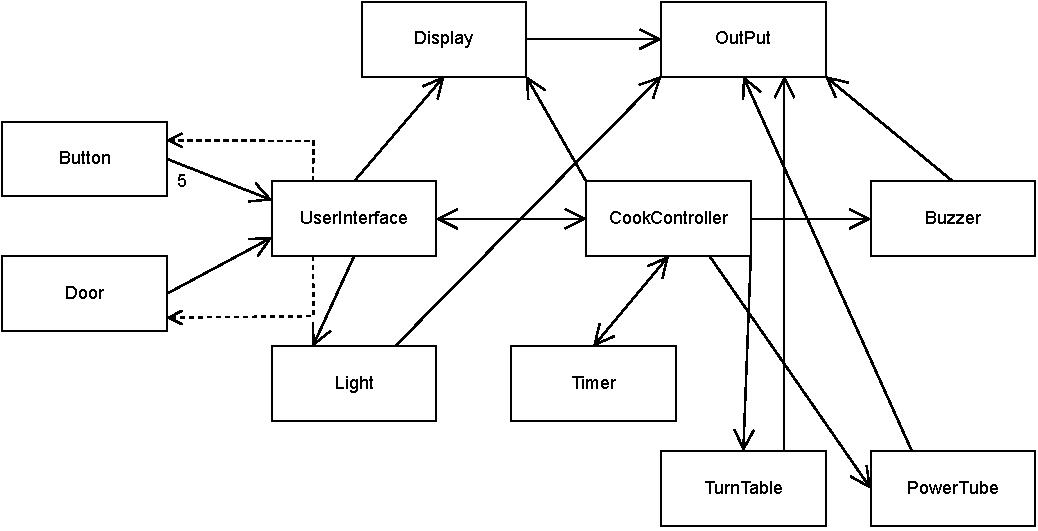
\includegraphics[scale=0.66]{02-Body/Image/ClassDiagram}
  \caption{Updated Class Diagram}%
  \label{fig:ClassDiagram}
\end{figure}
We have added two new classes. TurnTable and Buzzer.
The Buzzer has a uni directional association with the CookController class.
The TurnTable has a uni directional association with the CookControler and the Output class.
Lastly we added two more buttons to support the new features in the timer class.

\subsubsection{Short Description for Timer}
For the timer, we chose to make use of extra buttons to implement the adjust time features.
The buttons being a Increase Time Button and a Decrease time button. The user interface 
implements eventhandler for when these buttons are pushed. Classing the AdjustCookingTime
method in the CookController. Telling it to increase or decrease cooking time by 30 seconds.

The CookController itself calls an AdjustTime method in the timer class that increase or decrease
the time remaining by the requested amount.

\subsubsection{Short Description for Buzzer}
The buzzer is entirely controled by the buzzer, which can trun it on and off, as needed. This allows for easy addition of further use of the buzzer ( if e.g. it is desired to have a single buzz when the oven starts), without needing to alter anything other than the controller. We also added a property to allow the program to check if the buzzer is currently on. While this is currently only used in testing, it could be usefull to ensure that the buzzer is actually working as expected.

\subsubsection{Short Description for Power-Tube}
Since the power-tube max-power setting is set when setting up the power-tube module, the max-power is set in constructor and stored as a read-only. To change the hardcoded max-power the new max-power read-only-variable passed in the constructor of the UI module as well.

\subsubsection{Short Description for Turntable}
The new Turntable feature makes sure that the food in the microwaveoven rotates with the correct speed regarding the set power of the cooking program. The turntable can be started with a speed parameter and can be stopped. To calculate the correct speed the cookcontroller implements a new private method called “SpeedPowerConverter” that takes a “power” parameter and returns a “speed” parameter. 


\newpage

\subsection{STM Diagram UserInterface}
\begin{figure}[h]
  \centering
  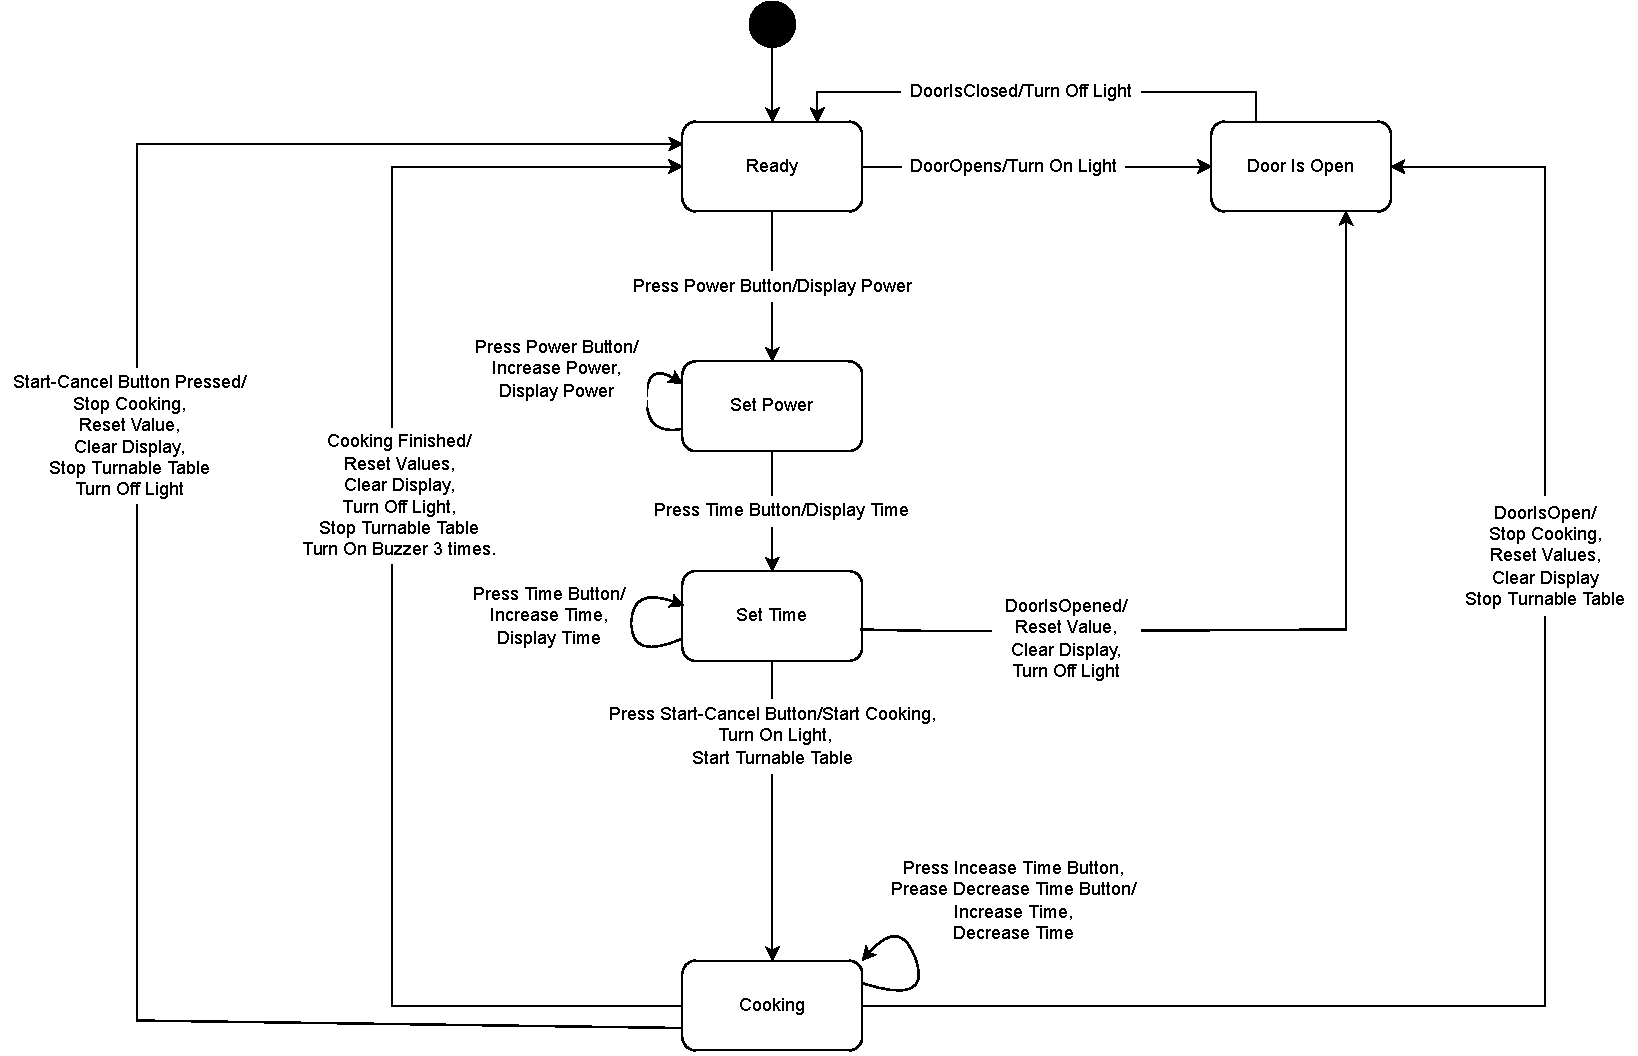
\includegraphics[scale=0.6]{02-Body/Image/STM_UserInterfacer.pdf}
  \caption{Updated STM diagram for UserInterface Class}%
  \label{fig:UserInterfaceSTM}
\end{figure}

\subsubsection{Changes Made to STM for UserInterface}.
Here follows a list of all changes made to the STM diagram for the UserInterface.

\begin{itemize}
  \item Start TurnTable when State: Set Time $=>$ Cooking
  \item Stop TurnTable when State: Cooknig $=>$ DoorIsOpen
  \item Stop TurnTable when State: Cooking $=>$ CookingFinished $=>$ Ready
  \item Stop TurnTable when State: Cooking $=>$ Cancel Button Pressed $=>$ Ready
  \item Increase/Decrease Time when State: Cooking
  \item Turn Buzzer On 3 times when State: Cooking $=>$ Cooking Finished $=>$ Ready 
\end{itemize}

\newpage
\begin{figure}[h]
  \centering
  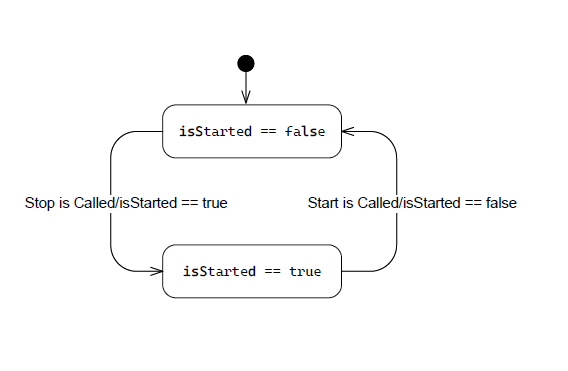
\includegraphics[scale=0.6]{02-Body/Image/TurntableSTM.PNG}
  \caption{STM diagram for Turntable}%
  \label{fig:TurntableSTM}
\end{figure}

\subsection{Sequence Diagram for Features}
\begin{figure}[h]
  \centering
  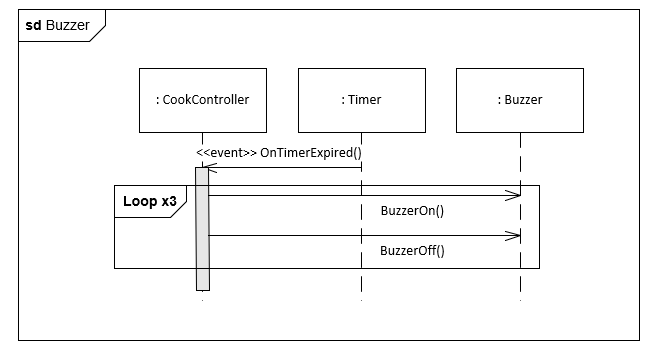
\includegraphics[scale=0.6]{02-Body/Image/BuzzerSEQ.PNG}
  \caption{Sequence diagram for CookController interacting with Buzzer}%
  \label{fig:BuzzerSeq}
\end{figure}

\begin{figure}[h]
  \centering
  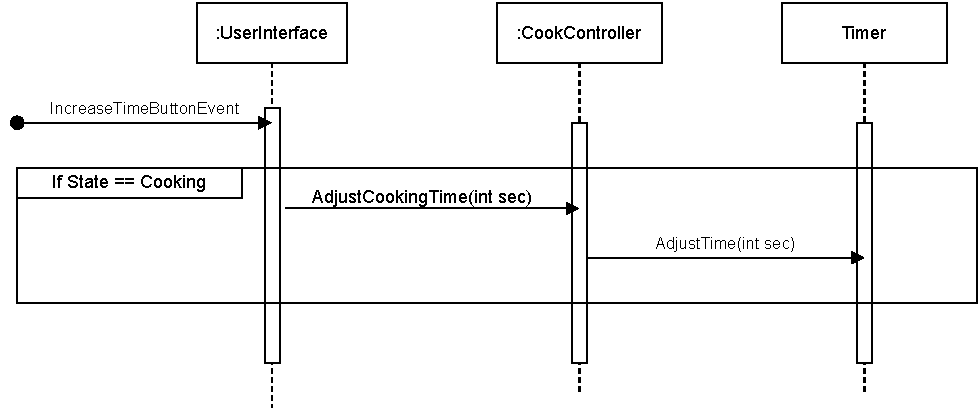
\includegraphics[scale=0.8]{02-Body/Image/TimerFeatureSEQ.pdf}
  \caption{Sequence Diagram for Timer Feature}%
  \label{fig:timeFeature}
\end{figure}

Here only the sequence diagram for the Increase time button has been added, since it
is identical for the decrease time button feature.

\begin{figure}[h]
  \centering
  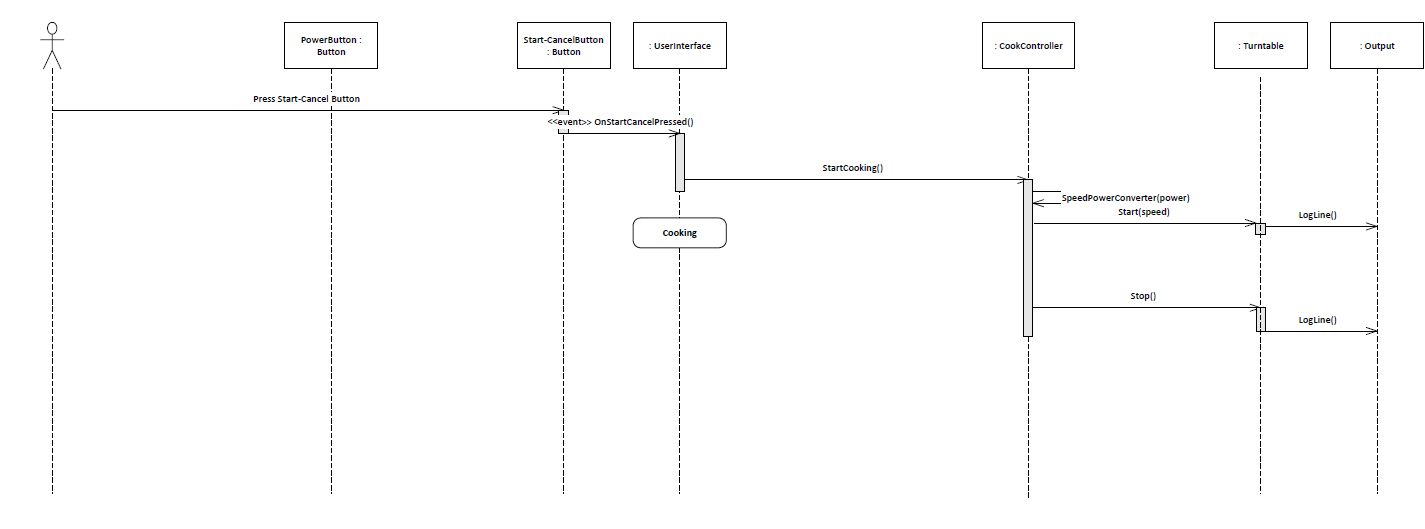
\includegraphics[scale=0.6]{02-Body/Image/TurntableSeq.PNG}
  \caption{Sequence diagram for Turntable interfacing with CookController}%
  \label{fig:TurntableSeq}
\end{figure}

\newpage
